\chapter{Premilinaries and Problem Definition}
\label{ch:premAndDef}


\section{The Friedkin and Johnsen Model}
\label{sec:prem}

The Friedkin-Johnsen model is a very popular opinion dynamic model \cite{friedkin}. This model uses information about the opinion of the user assuming there is an internal and external opinion. The internal opinions cannot change and is the specific opinion of an individual for a certain matter. On the other hand the expressed opinion is influenced by social interactions. The internal opinion of a user corresponds to the views that inherently holds for a controversial topic while the expressed opinion refers to the views that the user shares on a social network with his connections. The internal opinions of a user is denoted as $s_i$ and the expressed opinion as $z_i$.  
\\
\\
\begin{equation} 
	z_i = \frac{w_{ii}*si + \sum_{j \epsilon N(i) }{w_{ij}*z_j}} {w_{ii} + \sum_{j \epsilon N(i) }{w_{ij}}} 
\end{equation} 
\clearpage

\noindent The expressed opinion $z_i$ is computed as a weighted average of the external opinions of the neighbourhood of the user, for example, the opinions of the users friend list or the opinions of the accounts the user follows. The opinions of the users are stored in a vector $z$. The opinion vector $z$ is a metric for the whole social graph and can give us insights about its current situation. The vector values range from [-1,1]. Values closer to the range limits indicate bigger polarization. Polarized graphs create groups of nodes that are strongly connected with each other.
\\
\\
There are two ways of obtaining the $z$ vector of opinions. The first is to use repeated averaging until the model converges. An equivalent way is by computing the following: if $L$ is the laplacian matrix of a graph $G=(V,E)$, and $I$ is the identity matrix, then $z=(L+I)^{-1}S$ \cite{bindel}. 

\section{Measuring the polarization}
\label{sec:meas}

\noindent Let $G = (V,E)$ be a connected undirected graph representing a network. Let $z$ be the vector of expressed opinions  for the whole network. Each value  of the vector represents a node and can be computed with the opinion formation model of Friedkin-Johnsen. We use the definition of the polarization index \cite{tsapMatakosTerzi}. The polarization is measured by its distance from a neutral opinion.
\vspace{20pt}
\begin{equation}
	\pi(z) = ||z||_{2}^2
\end{equation}
\vspace{20pt}

\noindent To make the polarization index independent of its network we can normalize it by dividing it with the length of the vector $z$. 
\clearpage

\section{Problem Definition}
\label{sec:problemDef}

\noindent Problem 1 [k-Addition]. \noindent Let $G = (V,E)$ be a connected undirected graph representing a network and $k$ a given number of edges. Let $z$ be the vector of expressed opinions  for the whole network and $\pi(z) = ||z||_{2}^2$ the polarization index of this social graph. Let also $C \subseteq	V \times V$ set of edges that are not in the graph. We want to find a subset of $S \subseteq C$ of $k$ edges whose addition to a graph $G$ will reduce the polarization index $\pi(z)$.
\\
\\
\noindent Problem 1 is trying to find edges that will minimize the polarization index. We must not take for granted that these edges will be accepted. 
For example a social media user could reject a new follow/friend request. This leads us to consider additions with the expectation of being accepted. 
\\
\\
\noindent Problem 2 [K-Addition-Expected]. Let $G = (V,E)$ be a connected undirected graph representing a network and $k$ a given number of edges. Let $z$ be the vector of expressed opinions  for the whole network and $\pi(z) = ||z||_{2}^2$ the polarization index of this social graph. Let also $C \subseteq V \times V$ set of edges that are not in the graph and $P(u,v)$ a probability that the edge addition $u,v$ is accepted. We want to find a subset of $S \subseteq C$ of $k$ edges whose addition to a graph $G$ will show us how much we expect the polarization index $\pi(z)$ to be reduced.


\section{Monotonicity of the Problem}
\label{sec:monotonicity}

\begin{lemma}
The polarization index does not necessarily decrease after an edge addition between opposing views.
\end{lemma}

\vspace{20pt}
\noindent We will  show this with a counter example. In the network~\ref{fig:p5} nodes 0, 2 and 3 have a value of $s_i=-1$, and nodes 1 and 4 have a value of $s_i=+1$. For both examples we assume that $w_{ii}=w_{ij}=w_{ji}=1$ and $n$ the number of nodes. We will now compute the polarization index of the original graph
\\
\begin{figure}[h]
	\centering
	\begin{subfigure}[t]{0.3\textwidth}
		\centering
		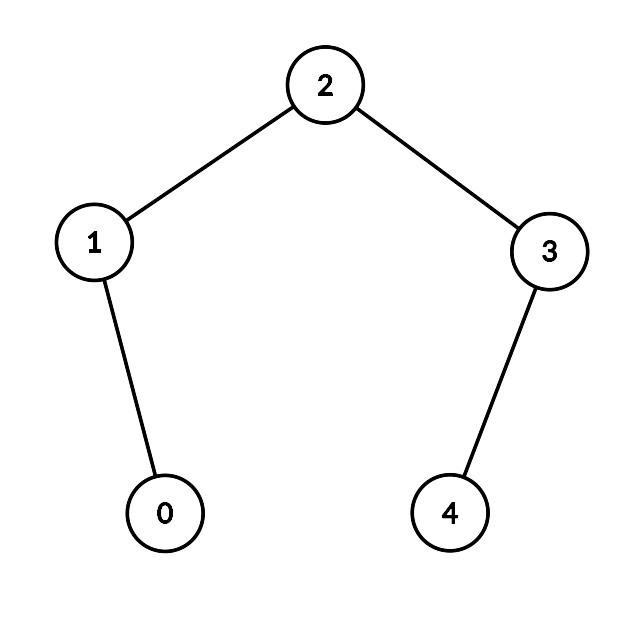
\includegraphics[height=0.15\textheight]{Figures/p5A}
		\caption{}
		\label{subfig:monotonicityA}
	\end{subfigure}
	\hfill
	\begin{subfigure}[t]{0.3\textwidth}
		\centering
		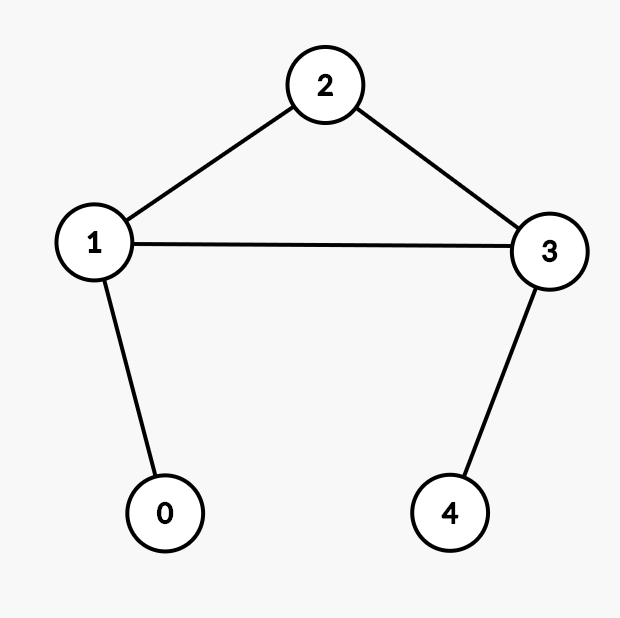
\includegraphics[height=0.15\textheight]{Figures/p5B}
		\caption{}
		\label{subfig:monotonicityB}
	\end{subfigure}
	\vspace{40pt}
	\hfill
	\caption{Edge addition between opposed opinions.}
	\label{fig:p5}
\end{figure}
\\

\begin{equation}
	\begin{aligned}
		(L+I)^{-1}s=z=
		\left(\begin{matrix}
		\frac{-27}{55} \\
		\frac{1}{55} \\
		\frac{-5}{11} \\
		\frac{-21}{55} \\
		\frac{17}{55}
		\end{matrix}\right),
		\qquad \qquad
		\pi(z)= 0.13785123966
	\end{aligned}
\end{equation}
\\
We will now compute the polarization index after the addition of the edge $1\rightarrow3$.

\begin{equation}
	\begin{aligned}
		(L+I)^{-1}s=z=
		\left(\begin{matrix}
		\frac{-53}{99} \\
		\frac{-7}{99} \\
		\frac{-5}{11} \\
		\frac{-29}{99} \\
		\frac{35}{99}
		\end{matrix}\right),
		\qquad \qquad
		\pi(z) = 0.14180185695
	\end{aligned}
\end{equation}
\\
\\
We can see an increase of the polarization index after adding this particular edge. This example was discovered after brute-forcing different graph topologies with different combinations of opinion values.
\clearpage

